


Na závěr teto bakalářské práce bych chtěl říct, že jsem měl radost pracovat nad velkým projektem, který má zkušeného vedoucího a projektového manažera. Zároveň, projekt je rozdělen do dvou častí, které se vyvíjí paralelně, což mi dalo možnost spolupracovat se skvělým programátorem během analýzy požadavku frontendové části.

Cílem teto práce je navržení vhodných úprav a následná implementace existujícího návrhu a fragmentů implementace. A také, zhodnocení použitelností výsledné implementace a navržení vhodných budoucích kroků pro pokračování vývoje serveru.

Práce se začíná analýzou existujícího návrhu a fragmentů implementace. I když jsem zúčastnil předmětů, které se zabývali těmto návrhem a implementací, potřeboval jsem přezkoumat celý návrh za účelem eliminování, nalezených během implementace frontendové a backendové častí, nedostatků a navržení lepších řešení.

Potom jsem návrh novou verzí řešení, která obsahuje úpravy podle požadavků frontendové části aplikace a zároveň obsahuje navržené mnou úpravy. Implementace navrženého řešení byla nejsložitější častí teto bakalářské práci, protože jsem neměl zkušeností ve vývoje projektů porovnatelného rozsahu a potřeboval jsem naučit mnoha novým věcem.
 
Následující důležitou částí teto práce bylo testování, které v rozsahu napsaného kódu je porovnatelnou s implementací serveru samotného. Provedl jsem analýzu počtu napsáných řádku kódu ve složce \textit{main} a \textit{test}. Pro počítaní řádek kódů jsem použil nástroj CLOC, který jsem zmínil v sekci \ref{reserse:cloc}. Na obrázku je \ref{image:code-count-test} zobrazen počet řádek kódu testů. Na obrázku je \ref{image:code-count-main} zobrazen počet řádek kódu implementace.
% \begin{figure}\centering
% 	   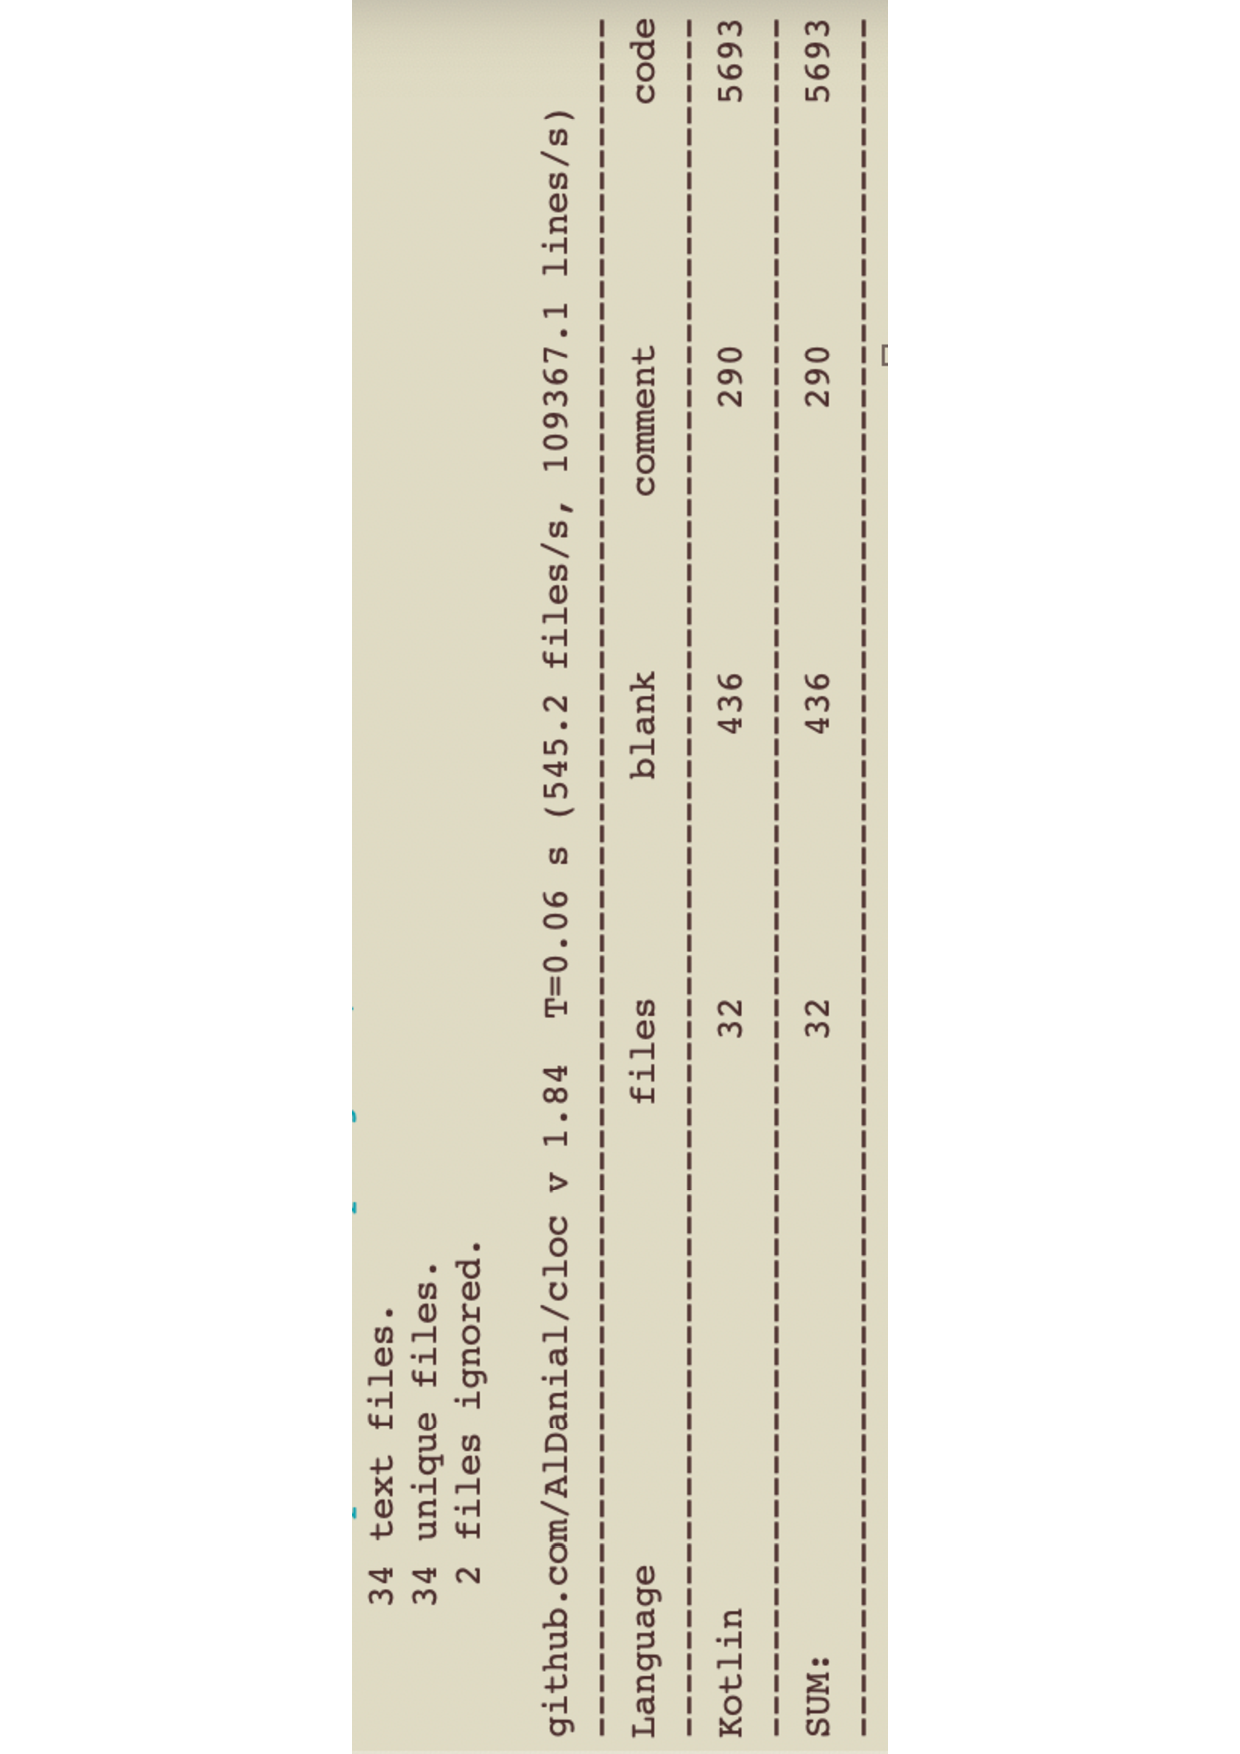
\includegraphics[angle=-90, width=0.5\textwidth]{pdfs/CodeAmountTests2}
% 	   \caption[Analýza kódu testů]{Počet napsáných řádek kódu testů}\label{image:code-count-test}
% \end{figure}
% \begin{figure}\centering
% 	   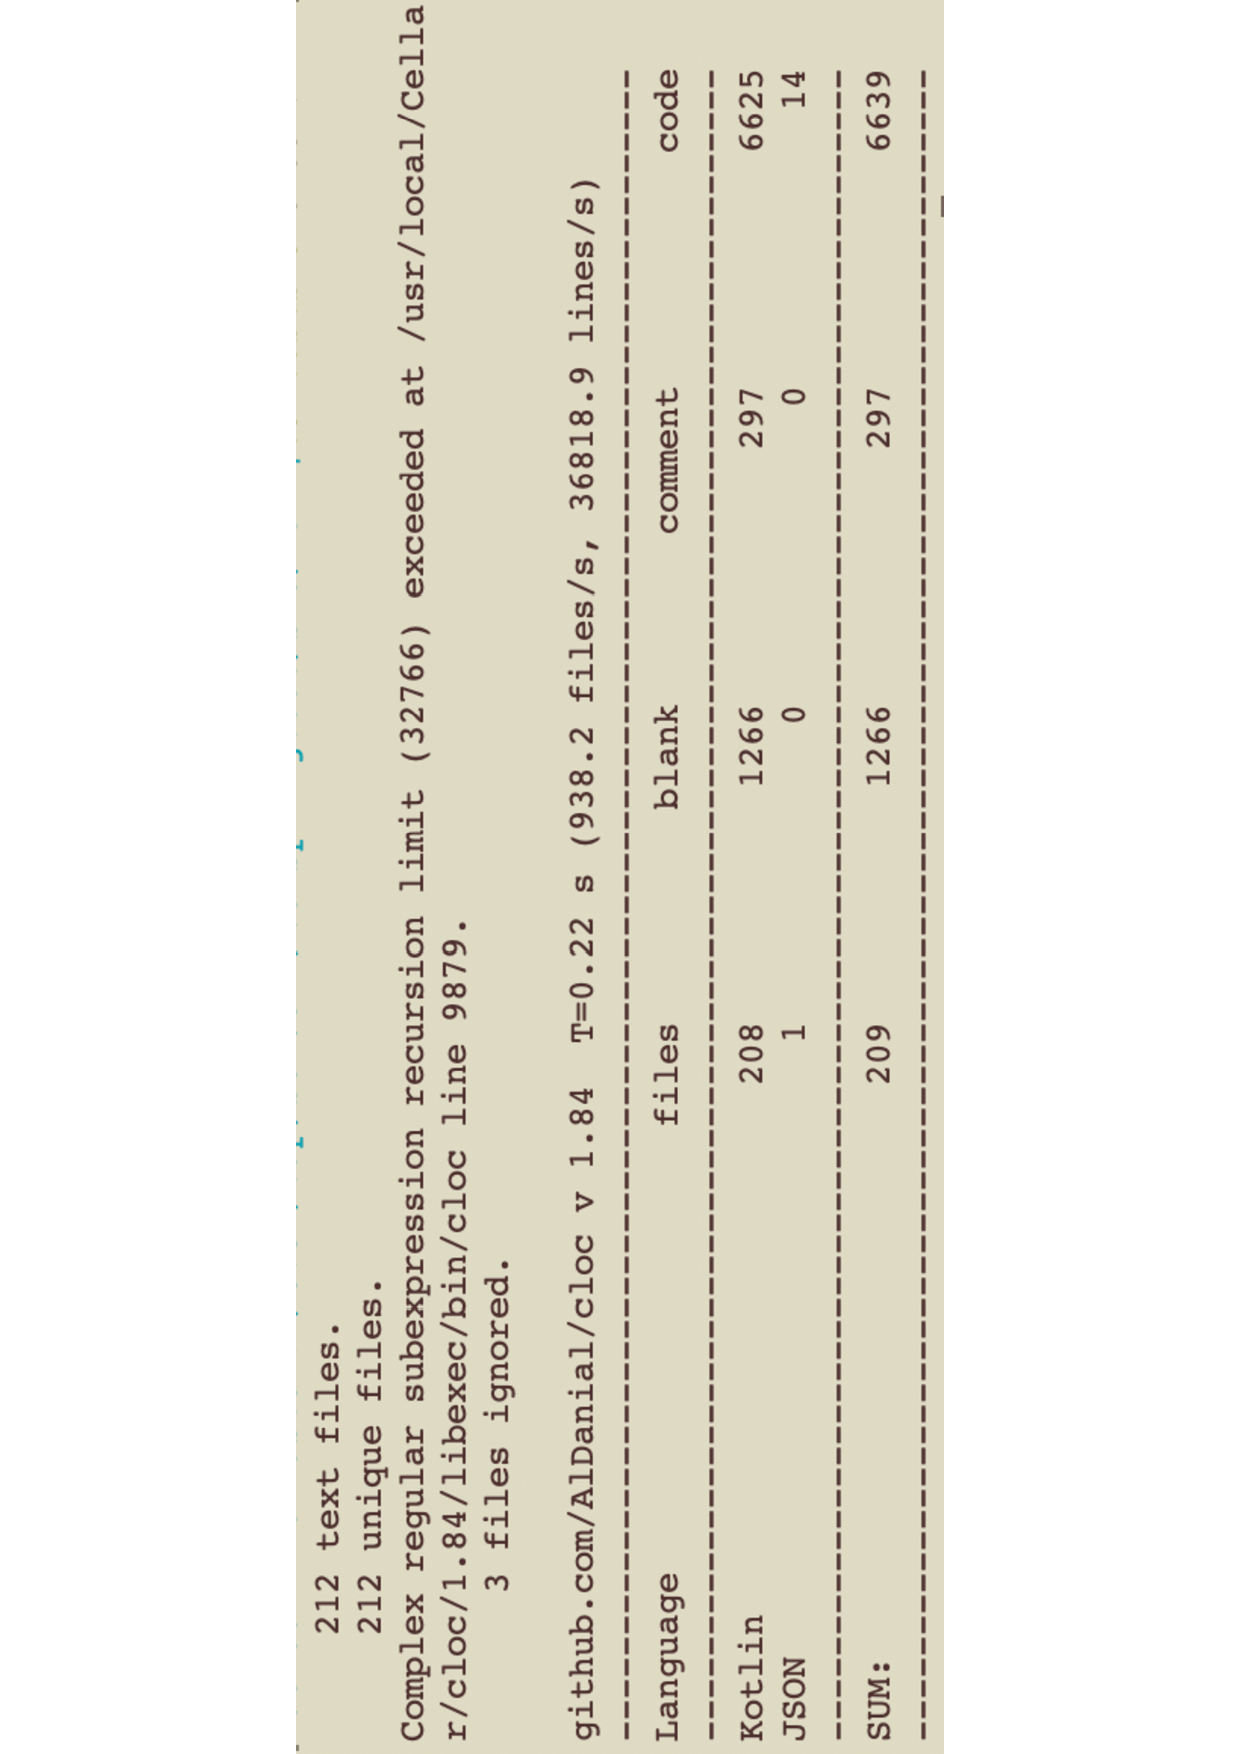
\includegraphics[angle=-90, width=0.5\textwidth]{pdfs/CodeAmountImpl2}
% 	   \caption[Analýza kódu implementace]{Počet napsáných řádek kódu za účelem implementace funkcionality}\label{image:code-count-main}
% \end{figure}

Následující kapitola se věnuje zhodnocení použitelností výsledné implementace a navržení budoucích kroků. Výsledek ještě není připravený pro produkční prostředí a ještě ho očekává dostatečný počet vylepšení. V rámci teto bakalářské práci jsem implementoval základ backendu, který má skoro celou potřebnou funkcionalitu, kromě některých věcí, které byly objevený už během pečlivého zanoření do implementace a za
řazené do budoucích kroků.